\documentclass[tikz]{standalone}
\begin{document}
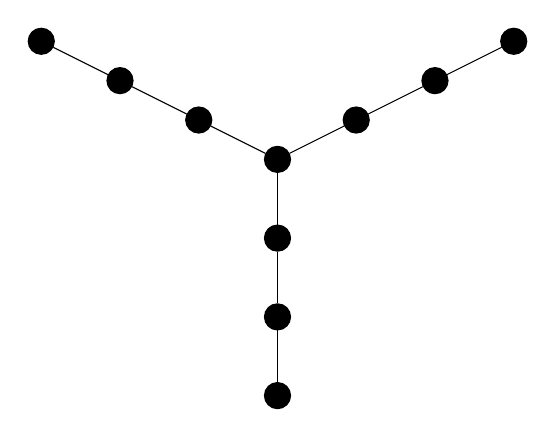
\begin{tikzpicture}

\node [draw, circle, fill=black] (v1) at (0,0) {};
\node [draw, circle, fill=black] (v2) at (0,-1) {};
\node [draw, circle, fill=black] (v3) at (0,-2) {};
\node [draw, circle, fill=black] (v4) at (0,-3) {};
\node [draw, circle, fill=black] (v5) at (-1,0.5) {};
\node [draw, circle, fill=black] (v8) at (1,0.5) {};
\node [draw, circle, fill=black] (v6) at (-2,1) {};
\node [draw, circle, fill=black] (v7) at (-3,1.5) {};
\node [draw, circle, fill=black] (v9) at (2,1) {};
\node [draw, circle, fill=black] (v10) at (3,1.5) {};
\draw  (v1) edge (v2);
\draw  (v2) edge (v3);
\draw  (v3) edge (v4);
\draw  (v1) edge (v5);
\draw  (v5) edge (v6);
\draw  (v6) edge (v7);
\draw  (v1) edge (v8);
\draw  (v8) edge (v9);
\draw  (v9) edge (v10);
\end{tikzpicture}
\end{document}